\documentclass{article}
\usepackage{times}
\usepackage{mcode}
\usepackage{graphicx}
\usepackage{caption}
\usepackage{subcaption}
\usepackage{mathtools}


\begin{document}
\title{Image Processing Exercise Book, TDT4195}
\author{Olav Olseng}
\maketitle
\newpage


\section*{Exercise 1}
\subsection*{Basic Image Processing}
\subsubsection*{Task 1}
I first read the images converting to doubles by typing into the "img" and "flatField" variables. I then use the imdivide function from the images toolbox to get a pixel-by-pixel division, and I store the result in my "res" variable. To show the result, i use the imshow function.

\begin{lstlisting}	
	img = im2double(imread('testimages/disturbed_potw1144a.png'))
	flatField = im2double(imread('testimages/flatfieldimage.png'))
	res = imdivide(img, flatField)
	imshow(res)
\end{lstlisting}
The images are loaded and normalized in a clamped double (values are between 0.0 and 1.0), with this loading function.
The finalized images look like this:
\\
\begin{figure}[h]
	\centering
	\begin{subfigure}[b]{0.45\textwidth}
		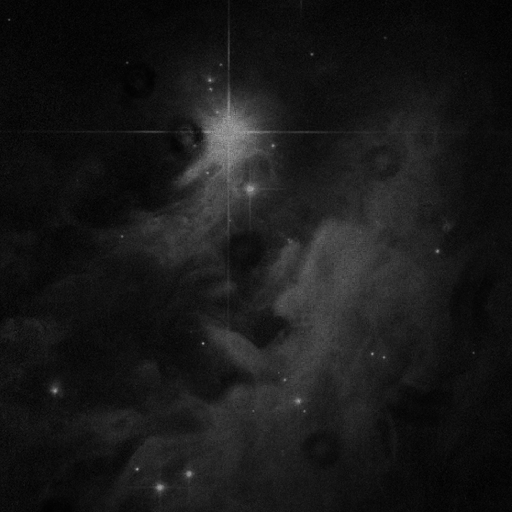
\includegraphics[width = \textwidth]{astro1.png}
		\caption{Original image}
		\label{fig:astro1.png}
	\end{subfigure}
	\begin{subfigure}[b]{ 0.45\textwidth}
		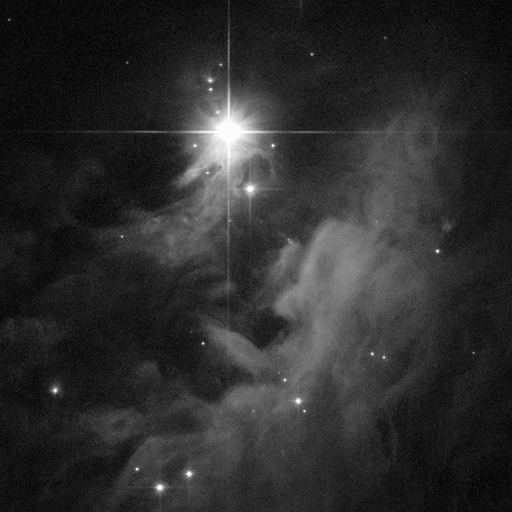
\includegraphics[width=\textwidth]{astro2.png}
		\caption{Processed image}
		\label{fig:astro2.png}
	\end{subfigure}
\end{figure}
\subsubsection*{Task 2}
We use division to \emph{increase} the gray-level, if we subract it becomes darker. This is due to the fact that the images are normalized withing [0.0, 1.0]. So the blacker the value of the flatfield image is, the brighter the result image will be in that particular pixel. This can however, create problems if the flatfield image has pixel values of 0 (completely black), as we might get division by zero.


\newpage
\subsection*{Filtering}
\subsubsection*{Task 1}
The image in the task is, at the time of writing, 17 pixels wide, not 16.\\ Original image:
\\
\begin{tabular}{|c|c|c|c|c|c|c|c|c|c|c|c|c|c|c|c|c|}
	\hline
	0 & 0 & 0 & 0 & 0 & 0 & 1 & 1 & 1 & 1 & 1 & 0 & 0 & 0 & 0 & 0 & 0 \\ 
	\hline
\end{tabular}
\paragraph{(a)}
The result i get from applying the filter to the 1D image is this:
\\
\begin{tabular}{|c|c|c|c|c|c|c|l|c|c|c|c|c|c|c|c|c|}
	\hline
	  &   & 0 & 0 & 1 & 2 & 3 & 4 & 5 & 4 & 3 & 2 & 1 & 0 & 0 &   &   \\ 
	\hline
\end{tabular}

\paragraph{(b)}
There isn't any need to apply extra padding in this example, it already seems to be padded with the six 0s on each side of the five 1s in the original image. So there isn't any real loss of data. This really depends on the implementation of the filter however.

\subsubsection*{Task 2}
If we do apply the continious convulution of this function we end up with:

\paragraph{(a)}
\begin{equation}
	\int_{-1/2}^{1/2} 1 \times 1 {d}v = 1
\end{equation}

\paragraph{(b)}
I expect this to give a the shape of a podium. Like they have in the olympics.

\newpage
\subsection*{Noise}
\subsubsection*{Task 1}

I chose the mandrill picture for this assignment. I applied the different salt \& pepper noise densities of 0.1, 0.3 and 0.5. \\
The noise was applied using the images toolbox function suggested in the assignment.
\begin{lstlisting}
	P = imnoise(I, 'salt & pepper', 0.1)
\end{lstlisting}

\begin{figure}[h]
	\centering
	\caption {Different salt and pepper noise densities}
	\begin{subfigure}[b]{0.3\textwidth}
		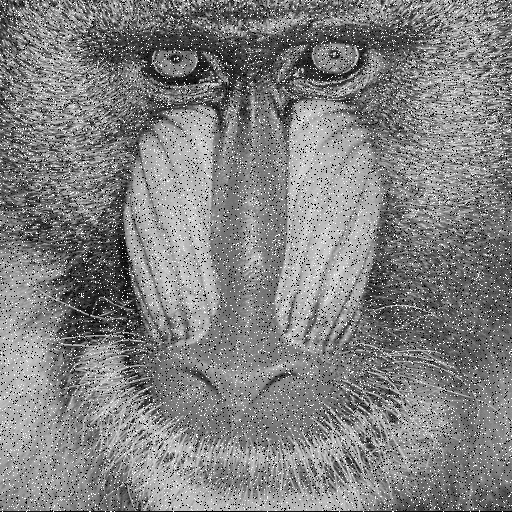
\includegraphics[width = \textwidth]{Mandrill01.png}
		\caption{0.1 Density}
		\label{fig:Mandrill01.png}
	\end{subfigure}
	\begin{subfigure}[b]{0.3\textwidth}
		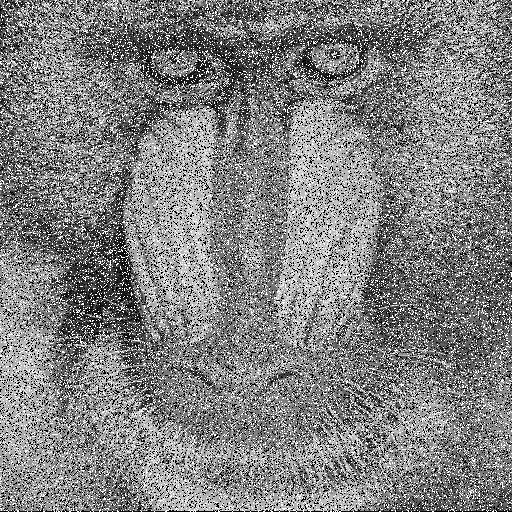
\includegraphics[width = \textwidth]{Mandrill03.png}
		\caption{0.3 Density}
		\label{fig:Mandrill03.png}
	\end{subfigure}
	\begin{subfigure}[b]{0.3\textwidth}
		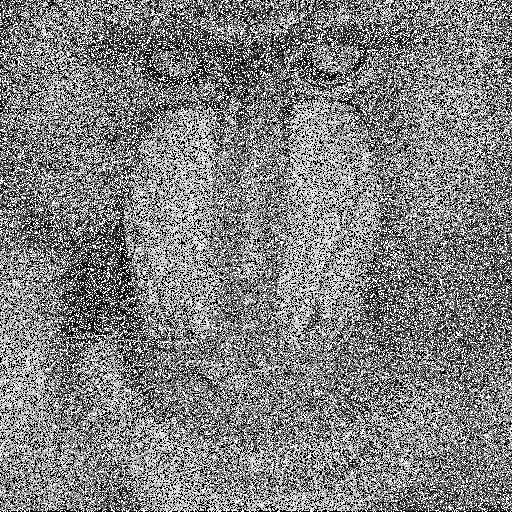
\includegraphics[width = \textwidth]{Mandrill05.png}
		\caption{0.5 Density}
		\label {fig:Mandrill05.png}
	\end{subfigure}
\end{figure}

Other noise types include, but not limited to, gaussian noise, uniform noise and exponential noise.

\newpage
\section*{Aliasing}
\subsection*{Task 1}
Here are the brick images with different sampling rates:\\

\begin{figure}[h]
	\centering
	\begin{subfigure}[t]{0.49\textwidth}
		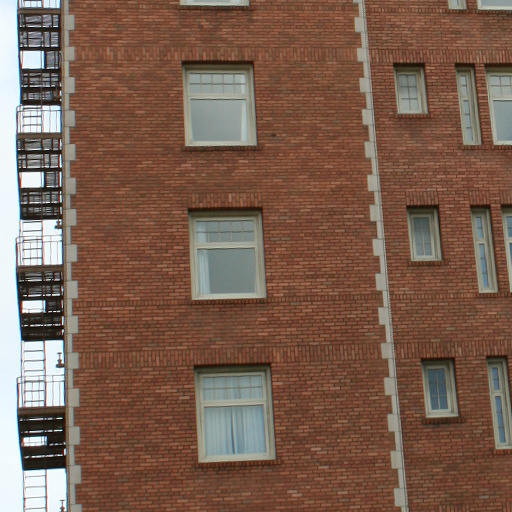
\includegraphics[width = \textwidth]{aliasbrick1.png}
		\caption{Original image}
		\label{fig:aliasbrick1.png}
	\end{subfigure}
	\begin{subfigure}[t]{0.49\textwidth}
		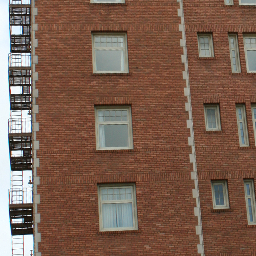
\includegraphics[width = \textwidth]{aliasbrick2.png}
		\caption{Half of image sampled}
		\label{fig:aliasbrick2.png}
	\end{subfigure}
	\begin{subfigure}[b]{0.49\textwidth}
		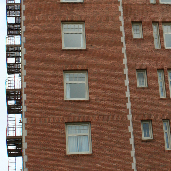
\includegraphics[width = \textwidth]{aliasbrick3.png}
		\caption{Third of image sampled}
		\label{fig:aliasbrick3.png}
	\end{subfigure}
	\begin{subfigure}[b]{0.49\textwidth}
		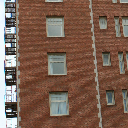
\includegraphics[width = \textwidth]{aliasbrick4.png}
		\caption{Fourth of  image sampled}
		\label{fig:aliasbrick4.png}
	\end{subfigure}
\end{figure}

As there is a pattern in the way the bricks a distributed in the wall, this pattern gets malformed as we downsample the image. Especially when we keep only a third and a fourth of the original data, we see new patterns emerge at the bottom of the wall.
This effect was not as prevalent when i did the same downsampling on the lena.png image. This might be due to the fact that the image of a woman, doesn't have such a mathematical pattern in it, as the brickwall does.



\end{document}
